\section{Introduction}\label{sec:chapter-1}

\subsection{Background and motivation}

A daily self-care routine involves several different activities: noticing a present feeling, choosing something manageable, completing that activity, and reflecting afterwards. When these activities are disconnected, the user must repeatedly decide where to begin. Holistic Mind brings them into one mobile environment. Its intended experience is a short, voluntary sequence of check-in, practice, feedback, and reflection, supported by an exercise catalogue and a separate learning library. This project treats that sequence as a software design problem. It does not assume that using an application produces a measurable improvement in mental health.

The original proposal focuses on adults seeking support with trauma-related difficulties, anxiety, and ADHD between professional appointments \citep{shrestha2026a}. The project is motivated by the difficulty of selecting relevant content from a general library. Someone seeking focus may need a different suggestion from someone reporting low energy or feeling overwhelmed. A category label alone cannot capture every distinction, while a ranking model cannot reliably interpret every personal concern. The application therefore combines structured answers with declared comfort preferences. Personalisation is designed to organise available practices and reduce selection effort, while keeping users free to browse, decline a suggestion, or report discomfort.

\subsection{Problem statement}

The central problem is to deliver a coherent daily wellness experience without making unexplained or overly confident recommendations. Three challenges shape the implementation. First, a new account has little behavioural history, creating a cold-start problem. Second, semantic relevance does not guarantee suitability: a description can match a user's state while involving a practice they wish to avoid. Third, reflective journals contain private information that should not automatically become recommendation data. Addressing these challenges requires coordinated interface, API, ranking, storage, and evaluation decisions rather than an isolated algorithm.

\subsection{Research questions}

RQ1 asks whether a hybrid of structured suitability rules and semantic matching improves top-four recommendation relevance over random, semantic-only, and rules-based alternatives on the project's authored scenarios. RQ2 asks whether explicitly declared comfort restrictions remain enforced throughout filtering, ranking, and fallback behaviour. RQ3 asks whether persistent reflective journaling can coexist with personalisation when journal decryption remains on the user's device. These questions are deliberately bounded: the first concerns offline ranking quality, the second concerns software policy enforcement, and the third concerns an implemented privacy boundary.

\subsection{Contribution and report structure}

The contribution is an integrated mobile artefact supported by reproducible evaluation files and documented development checks. It connects account management, onboarding, daily check-ins, recommendations, practice media, feedback, encrypted journals, and managed learning content. The dissertation integrates the original proposal, interim reports, and final progress review with the current implementation and saved evaluation evidence. Section 2 reviews relevant technical ideas; Section 3 defines objectives and scope; Sections 4 to 6 explain methodology, design, and implementation; Section 7 examines testing evidence; and Section 8 evaluates the contribution and future work.

\begin{figure}[htbp]
\centering
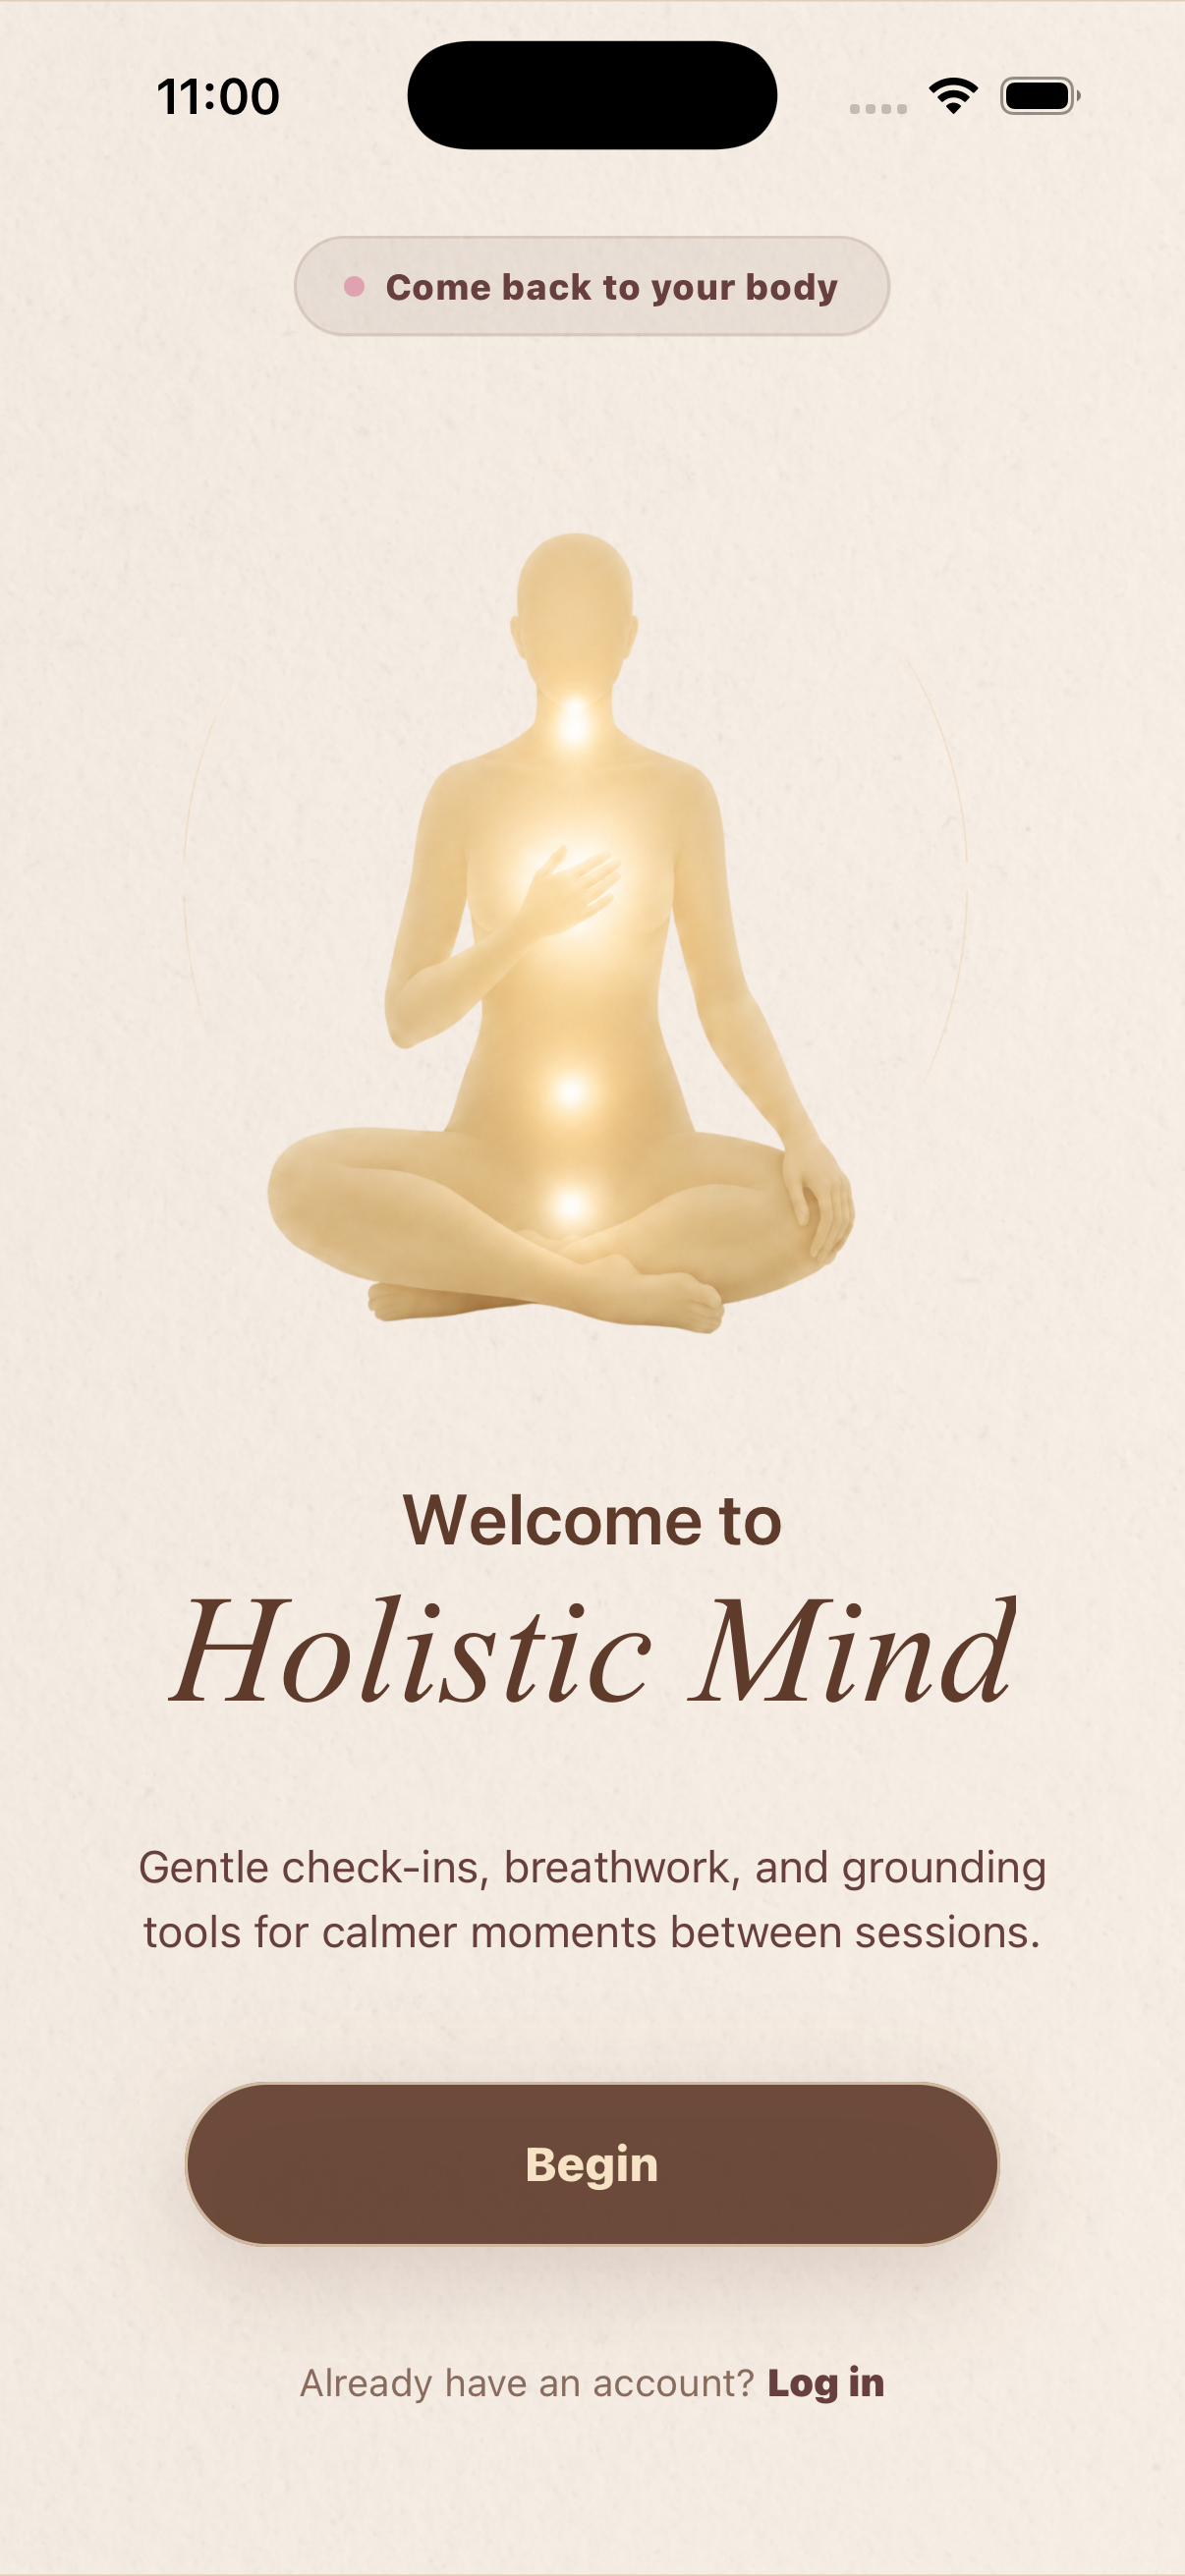
\includegraphics[width=\linewidth,height=0.62\textheight,keepaspectratio]{figures/welcome.png}
\caption[Welcome screen]{Existing iOS simulator welcome screen, captured 3 October 2026. The image illustrates the application's visual identity; it is not a usability-test result.}
\label{fig:welcome}
\end{figure}
\FloatBarrier

\subsection{Original motivation and intended users}

The proposal defined Holistic Mind as a trauma-informed mobile application for adults seeking support with childhood-trauma-related difficulties, anxiety, and ADHD between therapy sessions \citep{shrestha2026a}. That intended audience remains central to the project's design rationale. The application offers a private place to notice a current state, access a short practice, and reflect afterwards. The term trauma-informed describes an intention to respect choice, predictability, and personal comfort. It does not identify the software as a validated trauma treatment, and the application does not determine whether a user has trauma or ADHD.

The most useful element of the original proposal is its emphasis on the period between professional appointments. In that setting, a person may already have strategies they prefer but find it difficult to choose or remember one in a stressful moment. Holistic Mind organises a curated collection rather than expecting the person to search an unstructured information source. Its recommendations remain optional. A user can browse independently, avoid a particular type of practice, and provide feedback about an experience. This design addresses a concrete interaction problem while preserving the original supportive purpose.

The early proposal included a freemium commercial model and Firebase authentication. Later scope documentation placed subscription infrastructure outside the core academic deliverable. These changes distinguish the idea's commercial possibilities from what the final artefact actually implements. Likewise, the proposal's content counts describe intended delivery targets, not an audited inventory of the current catalogue. The benchmark's 14 exercises are evaluation fixtures, while the mobile application can display a larger managed catalogue. The report therefore avoids treating these different counts as interchangeable measures of completion.

\subsection{Project evolution across previous submissions}

The supplied reports form a useful sequence of decisions. The April interim report introduced a Design Science Research approach and a planned mixed-method study. The June progress review documented React Native selection, Firebase setup, initial authentication, and onboarding. Its supervisor questions asked whether a rule-based first version, explanation text, and comparison against random suggestions would be appropriate. The September final progress review then described a broader platform with custom authentication, PostgreSQL, a separate Python service, administration tools, and cloud-hosted content \citep{shrestha2026b,shrestha2026c,shrestha2026d}.

Current implementation extends that sequence with explicit comfort preferences and device-only journal encryption. The original ethical intention was that journals should not be analysed for modelling. An intermediate implementation used limited journal context, as the September review acknowledged. The present recommendation route restores a stronger separation by sending no journal text at all. This is a substantive change to the privacy and personalisation design, not merely a change in terminology. It also requires the journal-free benchmark rather than the earlier journal-containing results to represent current application inputs.

A final dissertation should explain this evolution instead of flattening every earlier statement into a claim about the final system. Firebase remains part of the documented prototype history. The September review's claim of a deployed beta describes that reported stage, while the later encrypted journal changes were verified locally and have a separate rollout status. The proposed five-participant study remains a planned activity unless participant records and analysis are supplied. These distinctions allow the original ambitions to remain visible without overstating their completion.
